\documentclass[14pt]{extbook}
\usepackage{multicol, enumerate, enumitem, hyperref, color, soul, setspace, parskip, fancyhdr} %General Packages
\usepackage{amssymb, amsthm, amsmath, latexsym, units, mathtools} %Math Packages
\everymath{\displaystyle} %All math in Display Style
% Packages with additional options
\usepackage[headsep=0.5cm,headheight=12pt, left=1 in,right= 1 in,top= 1 in,bottom= 1 in]{geometry}
\usepackage[usenames,dvipsnames]{xcolor}
\usepackage{dashrule}  % Package to use the command below to create lines between items
\newcommand{\litem}[1]{\item#1\hspace*{-1cm}\rule{\textwidth}{0.4pt}}
\pagestyle{fancy}
\lhead{Progress Quiz 8}
\chead{}
\rhead{Version A}
\lfoot{5493-4176}
\cfoot{}
\rfoot{Summer C 2021}
\begin{document}

\begin{enumerate}
\litem{
Choose the equation of the function graphed below.
\begin{center}
    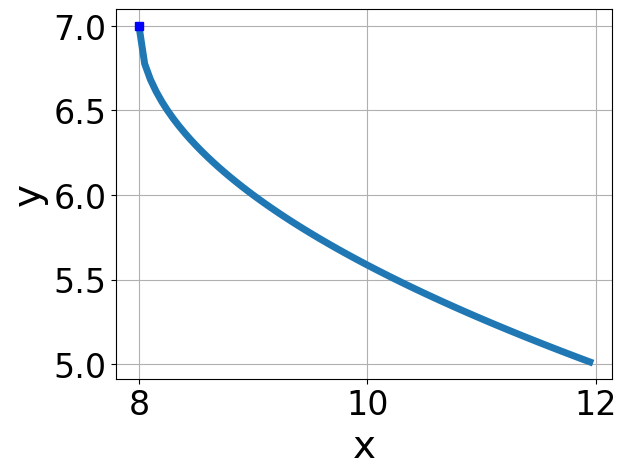
\includegraphics[width=0.5\textwidth]{../Figures/radicalGraphToEquationA.png}
\end{center}
\begin{enumerate}[label=\Alph*.]
\item \( f(x) = - \sqrt[3]{x - 8} + 7 \)
\item \( f(x) = - \sqrt[3]{x + 8} + 7 \)
\item \( f(x) = \sqrt[3]{x - 8} + 7 \)
\item \( f(x) = \sqrt[3]{x + 8} + 7 \)
\item \( \text{None of the above} \)

\end{enumerate} }
\litem{
Solve the radical equation below. Then, choose the interval(s) that the solution(s) belongs to.\[ \sqrt{-49 x^2 + 40} - \sqrt{-21 x} = 0 \]\begin{enumerate}[label=\Alph*.]
\item \( x \in [0.85,1.23] \)
\item \( x_1 \in [-0.89, -0.53] \text{ and } x_2 \in [-0.86,3.14] \)
\item \( x_1 \in [0.13, 1.01] \text{ and } x_2 \in [-0.86,3.14] \)
\item \( \text{All solutions lead to invalid or complex values in the equation.} \)
\item \( x \in [-0.89,-0.53] \)

\end{enumerate} }
\litem{
What is the domain of the function below?\[ f(x) = \sqrt[7]{8 x - 9} \]\begin{enumerate}[label=\Alph*.]
\item \( (-\infty, \infty) \)
\item \( \text{The domain is } (-\infty, a], \text{   where } a \in [0.82, 0.93] \)
\item \( \text{The domain is } [a, \infty), \text{   where } a \in [0.05, 0.96] \)
\item \( \text{The domain is } (-\infty, a], \text{   where } a \in [1.04, 1.86] \)
\item \( \text{The domain is } [a, \infty), \text{   where } a \in [1.03, 1.14] \)

\end{enumerate} }
\litem{
Choose the graph of the equation below.\[ f(x) = - \sqrt[3]{x - 14} + 6 \]\begin{enumerate}[label=\Alph*.]
\begin{multicols}{2}\item 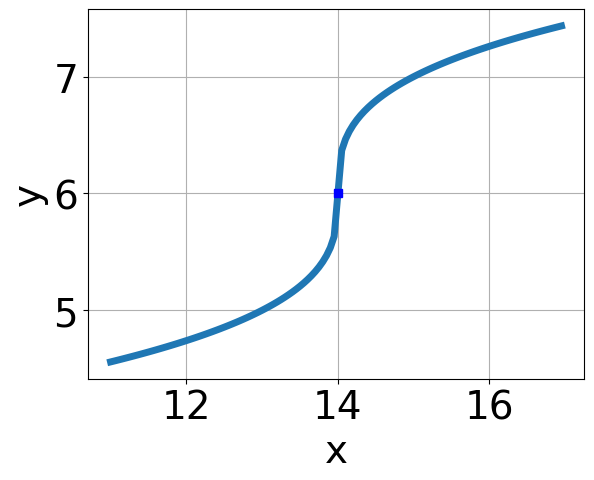
\includegraphics[width = 0.3\textwidth]{../Figures/radicalEquationToGraphCopyAA.png}\item 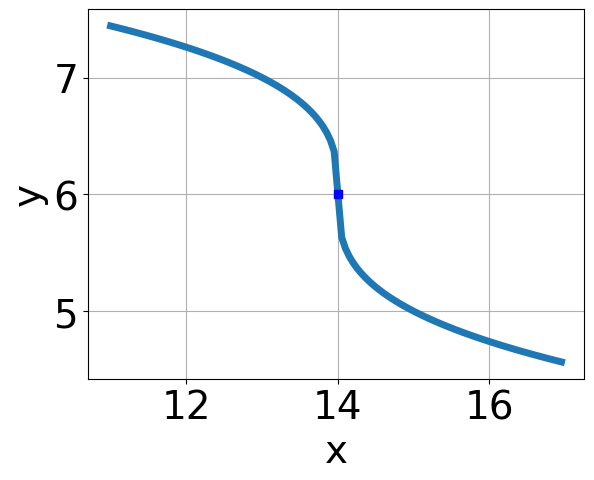
\includegraphics[width = 0.3\textwidth]{../Figures/radicalEquationToGraphCopyBA.png}\item 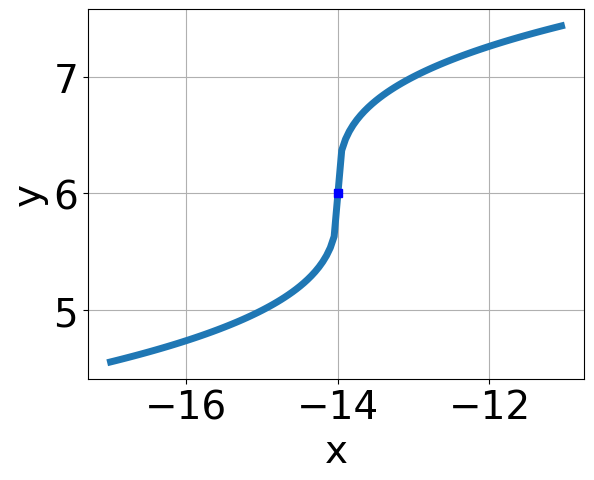
\includegraphics[width = 0.3\textwidth]{../Figures/radicalEquationToGraphCopyCA.png}\item 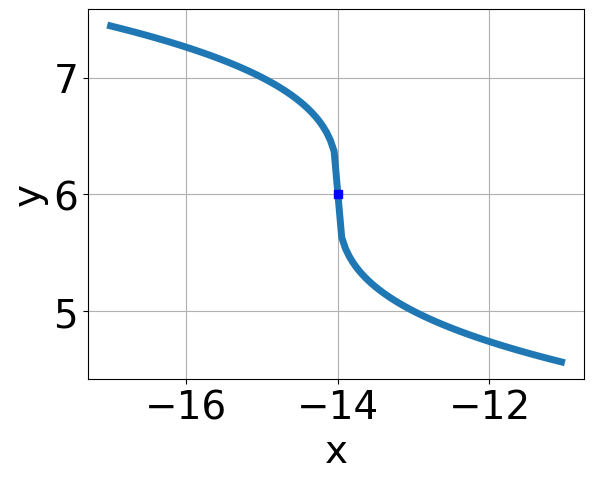
\includegraphics[width = 0.3\textwidth]{../Figures/radicalEquationToGraphCopyDA.png}\end{multicols}\item None of the above.
\end{enumerate} }
\litem{
Solve the radical equation below. Then, choose the interval(s) that the solution(s) belongs to.\[ \sqrt{-6 x + 5} - \sqrt{-3 x - 5} = 0 \]\begin{enumerate}[label=\Alph*.]
\item \( x \in [2.7,4.1] \)
\item \( x_1 \in [0.4, 1.5] \text{ and } x_2 \in [1.33,5.33] \)
\item \( x \in [-0.6,0.3] \)
\item \( \text{All solutions lead to invalid or complex values in the equation.} \)
\item \( x_1 \in [-3.3, -1.4] \text{ and } x_2 \in [-1.17,2.83] \)

\end{enumerate} }
\litem{
Choose the equation of the function graphed below.
\begin{center}
    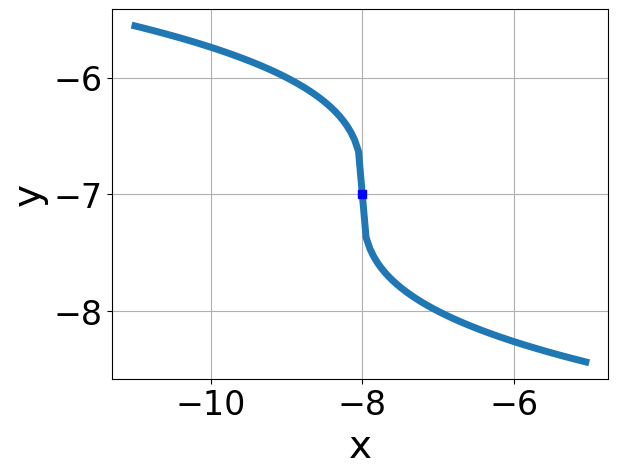
\includegraphics[width=0.5\textwidth]{../Figures/radicalGraphToEquationCopyA.png}
\end{center}
\begin{enumerate}[label=\Alph*.]
\item \( f(x) = \sqrt{x - 8} - 7 \)
\item \( f(x) = - \sqrt{x + 8} - 7 \)
\item \( f(x) = \sqrt{x + 8} - 7 \)
\item \( f(x) = - \sqrt{x - 8} - 7 \)
\item \( \text{None of the above} \)

\end{enumerate} }
\litem{
Solve the radical equation below. Then, choose the interval(s) that the solution(s) belongs to.\[ \sqrt{8 x - 7} - \sqrt{5 x + 5} = 0 \]\begin{enumerate}[label=\Alph*.]
\item \( x \in [0.4,0.75] \)
\item \( x \in [4,4.36] \)
\item \( x_1 \in [-1.21, -0.69] \text{ and } x_2 \in [-2.12,1.88] \)
\item \( x_1 \in [0.83, 1.02] \text{ and } x_2 \in [3,9] \)
\item \( \text{All solutions lead to invalid or complex values in the equation.} \)

\end{enumerate} }
\litem{
What is the domain of the function below?\[ f(x) = \sqrt[5]{-5 x - 9} \]\begin{enumerate}[label=\Alph*.]
\item \( (-\infty, \infty) \)
\item \( \text{The domain is } (-\infty, a], \text{   where } a \in [-1.9, -1.1] \)
\item \( \text{The domain is } (-\infty, a], \text{   where } a \in [-1.3, -0.3] \)
\item \( \text{The domain is } [a, \infty), \text{   where } a \in [-2.48, -0.56] \)
\item \( \text{The domain is } [a, \infty), \text{   where } a \in [-1.03, -0.07] \)

\end{enumerate} }
\litem{
Choose the graph of the equation below.\[ f(x) = - \sqrt{x - 6} + 4 \]\begin{enumerate}[label=\Alph*.]
\begin{multicols}{2}\item 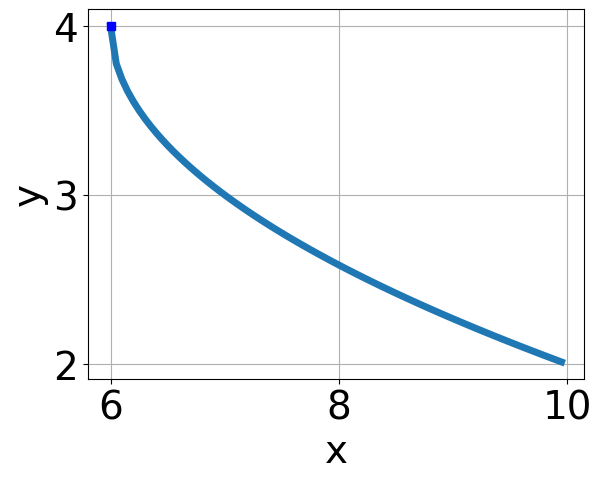
\includegraphics[width = 0.3\textwidth]{../Figures/radicalEquationToGraphAA.png}\item 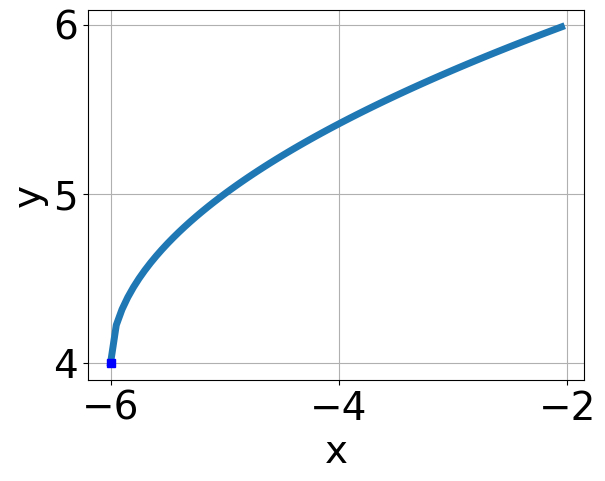
\includegraphics[width = 0.3\textwidth]{../Figures/radicalEquationToGraphBA.png}\item 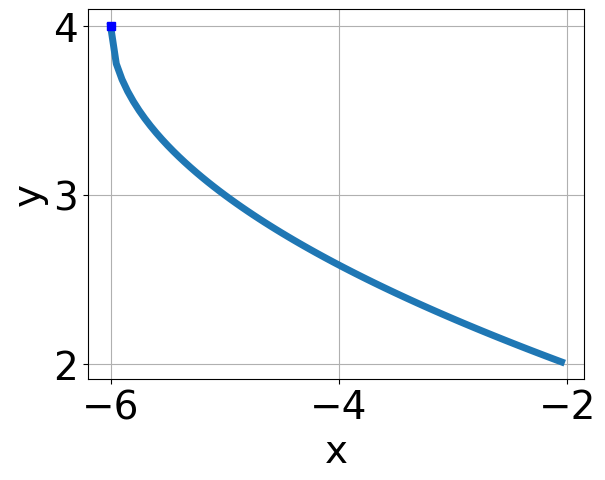
\includegraphics[width = 0.3\textwidth]{../Figures/radicalEquationToGraphCA.png}\item 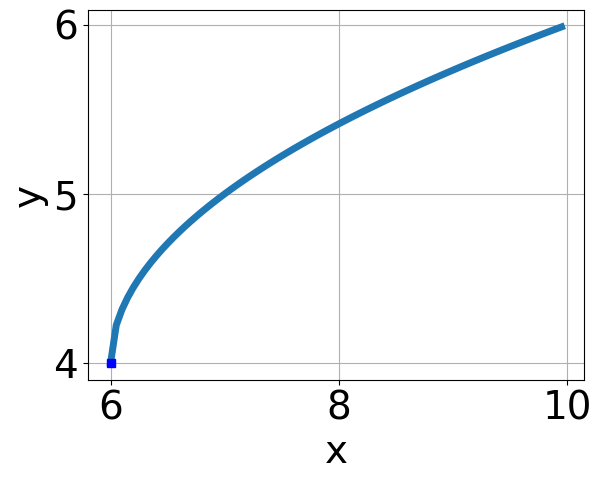
\includegraphics[width = 0.3\textwidth]{../Figures/radicalEquationToGraphDA.png}\end{multicols}\item None of the above.
\end{enumerate} }
\litem{
Solve the radical equation below. Then, choose the interval(s) that the solution(s) belongs to.\[ \sqrt{-35 x^2 + 54} - \sqrt{33 x} = 0 \]\begin{enumerate}[label=\Alph*.]
\item \( x \in [-3.9,-1] \)
\item \( x_1 \in [-0.1, 1] \text{ and } x_2 \in [1.56,2.76] \)
\item \( \text{All solutions lead to invalid or complex values in the equation.} \)
\item \( x_1 \in [-3.9, -1] \text{ and } x_2 \in [0.6,1.05] \)
\item \( x \in [-0.1,1] \)

\end{enumerate} }
\end{enumerate}

\end{document}